
\providecommand{\sSet}{s\mathcal{S}et}%
\providecommand{\qcThree}{\mathbf{3}} %
\providecommand{\rvTranspose}[1]{\ulcorner #1\urcorner}%
\providecommand{\QCat}{\mathcal{Q}\mathit{Cat}}%
\providecommand{\cellpair}[5]{$\vcenter{\hbox{\begin{tikzpicture}[x=1.15em,y=1.15em]%
\node (s) at (0,0) {$#1$};%
\node (t) at (4.2,0) {$#2$};%
\draw[->] (0.75,0.32) to[bend left=18] (3.45,0.32);%
\node at (2.1,0.88) {$\scriptstyle#3$};%
\draw[->] (0.75,-0.32) to[bend right=18] (3.45,-0.32);%
\node at (2.1,-0.93) {$\scriptstyle#4$};%
\draw[->] (1.95,0.2) to[bend right=32] (1.95,-0.2);%
\node at (2.85,0) {$\scriptstyle#5$};%
\end{tikzpicture}}}$\ignorespaces}

\section{笛卡尔与余笛卡尔纤维化}\label{sec:f-cartesian-cocartesian-fibrations}

本节的目标，是确立这样一些拟范畴之间的\trIsofibration{} $p\colon E\to B$ 的%
综合刻画与解析刻画之间的等价：它们定义\trCartesianFibration{}或%
\trCocartesianFibration。我们从考察 $p$-\trCartesianArrow{}入手，证明%
\cref{thm:pcartesian-characterizations}的三个综合定义与三个解析定义——后者
出现于 \cite[2.4.1.1, 2.4.1.4, 2.4.1.8]{bib78}——之间的等价。
随后，我们对\trCartesianFibration{}的综合刻画与解析刻画证明一个类似的比较，
并利用它来强化与\trCartesianFibration{}相关联的诸\trLifting{}性质。我们最后
证明：\trDiscreteCocartesianFibration{}与 Joyal 的\trLeftFibration{}相重合，而\trDiscreteCartesianFibration{}则与%
\trRightFibration{}相重合。

在 5.1 节中，「\trCartesianArrow」这一称谓指的是广义元素%
$\rvTranspose{\psi}\colon X\to E^{2}$，或者同样地，指它所表示的那个自然变换
\cellpair{X}{E}{e'}{e}{\psi}。在\trQuasiCategory{}的\trInfinityCosmos{}中，
一支 $X$-形箭头是\trCartesian，当且仅当它在每个\trElement{} $x\colon 1\to X$
处的诸分量 $\rvTranspose{\psi x}$ 都是\trCartesian{}（见%
\cref{prop:fiberwise-equivalence-cartesian-functor}）；于是，为简化下文的
讨论，我们只考虑形如 $\rvTranspose{\psi}\colon 1\to E^{2}$ 的箭头——亦即 $E$
中的 1-\trSimplex——并以简化记号 $\psi\colon e'\to e$ 来刻画它们。

\begin{proposition}\label{prop:cartesian-arrow-analytic}
固定拟范畴之间的一条\trIsofibration{} $p\colon E\twoheadrightarrow B$。以下诸条件等价，并且
刻画了 $E$ 中的 1-\trSimplex{} $\psi\colon e'\to e$ 何时是%
\textbf{$p$-\trCartesian}：
\begin{enumerate}[label=(\roman*)]
\item 由像为 $\qcThree$ 中\trCospan{} $0\to 2\leftarrow 1$ 的那个包含
$\delta\colon\llcorner\hookrightarrow\qcThree$ 所诱导的\trIsofibration
\begin{center}
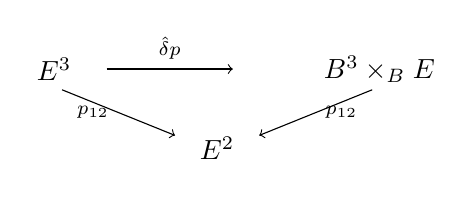
\begin{tikzpicture}[x=1.9em,y=1.5em]
  \node (E3) at (0,0)      {$E^{3}$};
  \node (Bp) at (6.2,0)    {$B^{3}\times_{B^{\llcorner}}E^{\llcorner}$};
  \node (E2) at (3.1,-1.9) {$E^{2}$};
  \draw[->] (1.0,0) -- node[above]{$\scriptstyle\hat{\delta}p$} (3.4,0);
  \draw[->] (0.15,-0.5) -- node[left]{$\scriptstyle p_{12}$} (2.3,-1.6);
  \draw[->] (6.05,-0.5) -- node[right]{$\scriptstyle p_{12}$} (3.9,-1.6);
\end{tikzpicture}
\end{center}
经拉回便在 $\psi$ 之上的\trFiber{}上定义一条\trTrivialFibration。
\item 如下左图的交换三角形定义了一个\trAbsoluteRightLifting{}图表
\begin{center}
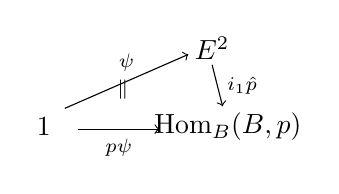
\begin{tikzpicture}[x=1.9em,y=1.5em]
  \node (o)  at (0,0)     {$1$};
  \node (E2) at (3.2,1.9) {$E^{2}$};
  \node (H)  at (3.5,0)   {$\mathrm{Hom}_{B}(B,p)$};
  \draw[->] (0.4,0.45) -- node[above,pos=0.5]{$\scriptstyle\psi$} (2.75,1.75);
  \node at (1.5,0.9) {$\scriptstyle\parallel$};
  \draw[->] (0.65,-0.05) -- node[below]{$\scriptstyle p\psi$} (2.2,-0.05);
  \draw[->] (3.2,1.5) -- node[right]{$\scriptstyle i_{1}\hat{p}$} (3.4,0.5);
\end{tikzpicture}
\quad 其中\quad
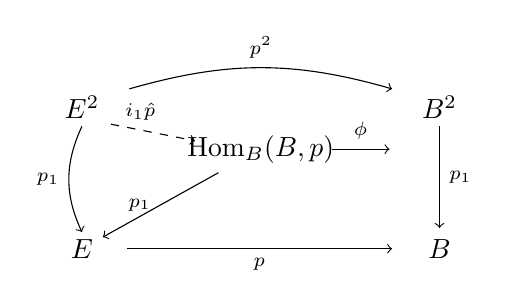
\begin{tikzpicture}[x=1.9em,y=1.5em]
  \node (E2) at (0,1.9)   {$E^{2}$};
  \node (B2) at (6.8,1.9) {$B^{2}$};
  \node (H)  at (3.4,0.9) {$\mathrm{Hom}_{B}(B,p)$};
  \node (E)  at (0,-1.5)  {$E$};
  \node (B)  at (6.8,-1.5){$B$};
  \draw[->] (0.9,2.35) to[bend left=16] node[above]{$\scriptstyle p^{2}$} (5.9,2.35);
  \draw[->,dashed] (0.55,1.5) -- node[above,pos=0.35]{$\scriptstyle i_{1}\hat{p}$} (2.15,1.1);
  \draw[->] (4.75,0.9) -- node[above]{$\scriptstyle\rvTranspose{\phi}$} (5.85,0.9);
  \draw[->] (0,1.45) to[bend right=25] node[left,pos=0.5]{$\scriptstyle p_{1}$} (0,-1.1);
  \draw[->] (H) -- node[left]{$\scriptstyle p_{1}$} (E);
  \draw[->] (6.8,1.45) -- node[right]{$\scriptstyle p_{1}$} (6.8,-1.0);
  \draw[->] (0.85,-1.5) -- node[below]{$\scriptstyle p$} (5.9,-1.5);
  \node at (3.9,0.5) {$\scriptstyle\llcorner$};
\end{tikzpicture}
\end{center}
\item 存在一个\trAbsoluteRightLifting{}图表，满足 $p_{1}\epsilon=\psi$ 与
$p_{0}\epsilon=\mathrm{id}_{pe'}$：
\begin{center}
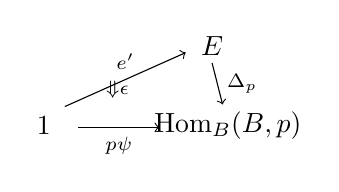
\begin{tikzpicture}[x=1.9em,y=1.5em]
  \node (o)  at (0,0)   {$1$};
  \node (E)  at (3.2,1.9) {$E$};
  \node (H)  at (3.5,0) {$\mathrm{Hom}_{B}(B,p)$};
  \draw[->] (0.4,0.45) -- node[above,pos=0.5]{$\scriptstyle e'$} (2.7,1.75);
  \node at (1.4,0.85) {$\scriptstyle\Downarrow\epsilon$};
  \draw[->] (0.65,-0.05) -- node[below]{$\scriptstyle p\psi$} (2.2,-0.05);
  \draw[->] (3.2,1.5) -- node[right]{$\scriptstyle\Delta_{p}$} (3.4,0.5);
\end{tikzpicture}
\quad 其中\quad
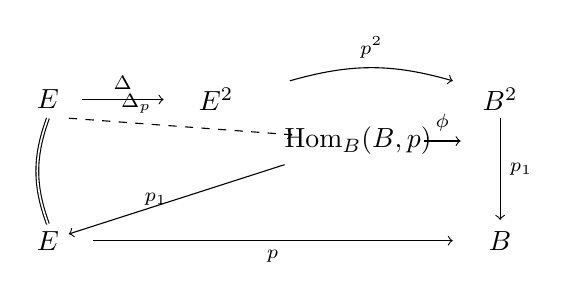
\begin{tikzpicture}[x=1.9em,y=1.5em]
  \node (E1) at (0,1.9)   {$E$};
  \node (E2) at (3.2,1.9) {$E^{2}$};
  \node (B2) at (8.6,1.9) {$B^{2}$};
  \node (H)  at (5.9,0.9) {$\mathrm{Hom}_{B}(B,p)$};
  \node (Eb) at (0,-1.5)  {$E$};
  \node (B)  at (8.6,-1.5){$B$};
  \draw[->] (0.65,1.9) -- node[above]{$\scriptstyle\Delta$} (2.2,1.9);
  \draw[->] (4.6,2.35) to[bend left=16] node[above]{$\scriptstyle p^{2}$} (7.7,2.35);
  \draw[->,dashed] (0.4,1.45) -- node[above,pos=0.3]{$\scriptstyle\Delta_{p}$} (4.65,1.05);
  \draw[->] (7.15,0.9) -- node[above]{$\scriptstyle\rvTranspose{\phi}$} (7.85,0.9);
  \draw[double] (0,1.45) to[bend right=20] (0,-1.1);
  \draw[->] (H) -- node[left]{$\scriptstyle p_{1}$} (Eb);
  \draw[->] (8.6,1.45) -- node[right]{$\scriptstyle p_{1}$} (8.6,-1.0);
  \draw[->] (0.85,-1.5) -- node[below]{$\scriptstyle p$} (7.7,-1.5);
  \node at (6.35,0.5) {$\scriptstyle\llcorner$};
\end{tikzpicture}
\end{center}
\item 方块
\begin{center}
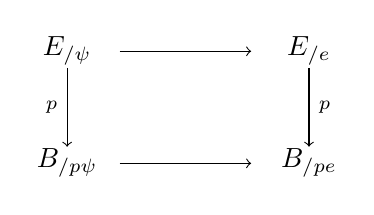
\begin{tikzpicture}[x=1.9em,y=1.5em]
  \node (Ep) at (0,1.3)   {$E_{/\psi}$};
  \node (Ee) at (4.6,1.3) {$E_{/e}$};
  \node (Bp) at (0,-1.4)  {$B_{/p\psi}$};
  \node (Be) at (4.6,-1.4){$B_{/pe}$};
  \draw[->] (1.0,1.3) -- (3.5,1.3);
  \draw[->] (0,0.9) -- node[left]{$\scriptstyle p$} (0,-1.0);
  \draw[->] (4.6,0.9) -- node[right]{$\scriptstyle p$} (4.6,-1.0);
  \draw[->] (1.0,-1.4) -- (3.5,-1.4);
\end{tikzpicture}
\end{center}
中到拉回的诱导映射是一条\trTrivialFibration{}
$E_{/\psi}\twoheadrightarrow B_{/p\psi}\mathbin{\underset{B_{/pe}}{\times}}E_{/e}$。
\item 任何 $n\ge 2$ 的如下形式的\trLifting{}问题都有解：
\begin{rveq}\label{eq:pcartesian-horn-lifting}
\begin{tikzpicture}[x=1.9em,y=1.4em]
  \node (d1) at (0,1.3)    {$\Delta[1]$};
  \node (ho) at (3.6,1.3)  {$\Lambda^{n}[n]$};
  \node (E)  at (7.4,1.3)  {$E$};
  \node (dn) at (3.6,-1.4) {$\Delta[n]$};
  \node (B)  at (7.4,-1.4) {$B$};
  \draw[->] (1.0,1.3) -- node[below]{$\scriptstyle\{n-1,n\}$} (2.6,1.3);
  \draw[->] (4.6,1.3) -- (6.4,1.3);
  \draw[->] (0.6,1.8) to[bend left=20] node[above,pos=0.5]{$\scriptstyle\psi$} (6.8,1.8);
  \draw[right hook->] (3.6,0.95) -- (3.6,-0.9);
  \draw[->,dashed] (4.0,-1.2) -- (6.9,1.0);
  \draw[->] (7.4,0.95) -- node[right]{$\scriptstyle p$} (7.4,-0.9);
  \draw[->] (4.6,-1.4) -- (6.4,-1.4);
\end{tikzpicture}
\end{rveq}
\item 任何 $n\ge 1$ 的如下形式的\trLifting{}问题都有解：
\begin{rveq}\label{eq:pcartesian-cylinder-lifting}
\begin{tikzpicture}[x=1.9em,y=1.4em]
  \node (d1)  at (0,1.3)    {$\Delta[1]$};
  \node (pd)  at (3.9,1.3)  {$\partial\Delta[n]\times\Delta[1]$};
  \node (d11) at (8.1,1.3)  {$\Delta[n]\times\{1\}$};
  \node (E)   at (10.9,1.3) {$E$};
  \node (dn)  at (5.0,-1.4) {$\Delta[n]\times\Delta[1]$};
  \node (B)   at (10.9,-1.4){$B$};
  \draw[->] (0.9,1.3) -- node[below]{$\scriptstyle\{n\}\times\mathrm{id}$} (2.3,1.3);
  \draw[->] (6.1,1.3) -- (6.9,1.3);
  \draw[->] (9.4,1.3) -- (10.2,1.3);
  \node at (6.0,1.8) {$\scriptstyle\sqcup$};
  \node at (6.0,0.7) {$\scriptstyle\partial\Delta[n]\times\{1\}$};
  \draw[->] (1.0,1.9) to[bend left=18] node[above,pos=0.45]{$\scriptstyle\psi$} (10.3,1.9);
  \draw[right hook->] (5.0,0.95) -- (5.0,-0.9);
  \draw[->,dashed] (5.5,-1.2) -- (10.4,1.0);
  \draw[->] (10.9,0.95) -- node[right]{$\scriptstyle p$} (10.9,-0.9);
  \draw[->] (6.8,-1.4) -- (9.9,-1.4);
\end{tikzpicture}
\end{rveq}
\end{enumerate}
\end{proposition}

\begin{proof}
\cref{thm:pcartesian-characterizations}在任何\trInfinityCosmos{}中证明了条件
(i)、(ii) 与 (iii) 的等价性。

由\cref{lem:dashed-square-hypercube}，(i) 中的映射同构于如下方块中到拉回的
诱导映射——该方块与 (iv) 中出现的方块十分相似。\footnote{诚然，方块
\eqref{eq:hypercube-weakly-cartesian} 中的始对象是一个我们记作 $E_{/\psi}$ 的
拟范畴，因为它\trEquivalence{}（尽管不同构）于 Joyal 的切片拟范畴（见
\cref{war:slice-notation}）。为免此处混淆，我们以 $E_{//\psi}$ 记该拟范畴，
而把记号 $E_{/\psi}$ 留给\cref{def:join}的切片拟范畴。}我们将通过在每一个%
\trWeaklyCartesianSquare{}中构造其顶行映射之间的、如下左侧所示的自然等价，来
证明这两个方块等价：
\begin{center}
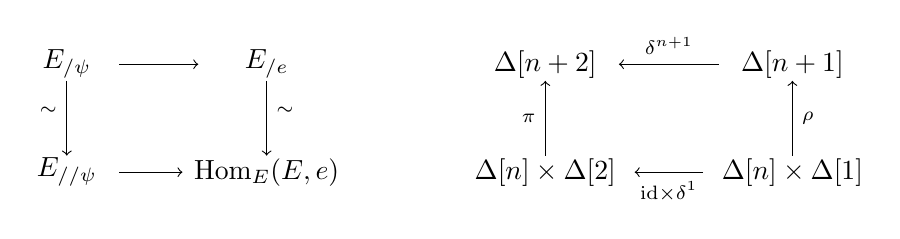
\begin{tikzpicture}[x=1.9em,y=1.5em]
  \node (l1) at (0,1.3)    {$E_{/\psi}$};
  \node (l2) at (3.8,1.3)  {$E_{/e}$};
  \node (l3) at (0,-1.3)   {$E_{//\psi}$};
  \node (l4) at (3.8,-1.3) {$\mathrm{Hom}_{E}(E,e)$};
  \draw[->] (1.0,1.3) -- (2.5,1.3);
  \draw[->] (0,0.9) -- node[left,pos=0.4]{$\scriptstyle\sim$} (0,-0.9);
  \draw[->] (3.8,0.9) -- node[right,pos=0.4]{$\scriptstyle\sim$} (3.8,-0.9);
  \draw[->] (1.0,-1.3) -- (2.2,-1.3);
  \node at (5.5,0) {$\;\leftrightsquigarrow\;$};
  \begin{scope}[shift={(7.2,0)}]
    \node (r1) at (1.9,1.3)  {$\Delta[n+2]$};
    \node (r2) at (6.6,1.3)  {$\Delta[n+1]$};
    \node (r3) at (1.9,-1.3) {$\Delta[n]\times\Delta[2]$};
    \node (r4) at (6.6,-1.3) {$\Delta[n]\times\Delta[1]$};
    \draw[->] (5.2,1.3) -- node[above]{$\scriptstyle\delta^{n+1}$} (3.3,1.3);
    \draw[->] (1.9,-0.9) -- node[left]{$\scriptstyle\pi$} (1.9,0.9);
    \draw[->] (6.6,-0.9) -- node[right]{$\scriptstyle\rho$} (6.6,0.9);
    \draw[->] (4.9,-1.3) -- node[below]{$\scriptstyle\mathrm{id}\times\delta^{1}$} (3.6,-1.3);
  \end{scope}
\end{tikzpicture}
\end{center}
此图中的诸映射，最容易借助它们在 $n$-\trSimplex{}上的作用来描述：每个映射都
沿上方右侧所示交换方块中相应的函子作限制而给出，其中 $\pi$ 与 $\rho$ 均由
如下公式定义：
\[
\rho(i,j)\coloneqq\pi(i,j)\coloneqq
\begin{cases}
i & j=0\\
n+j & j>0
\end{cases}
\]
\cref{prop:fat-join-comparison-weak-equivalence}与%
\cref{prop:slices-cones-equivalence}证明左手竖直映射是一个\trEquivalence，而
\cref{cor:slice-cone-point}则证明右手竖直映射是一个\trEquivalence。于是，这
两个方块等价，从而由\cref{lem:dashed-square-hypercube}，(i) 等价于 (iv)。

由\cref{prop:join-slice-adjunction}之\trAdjunction，刻画 (iv) 之%
\trTrivialFibration{}的那个\trLifting{}性质经转置便成为 (v) 的\trLifting{}%
性质
\begin{center}
\begin{tikzpicture}[x=1.9em,y=1.5em]
  \node (a) at (0,1.3)    {$\partial\Delta[n]$};
  \node (b) at (3.8,1.3)  {$E_{/\psi}$};
  \node (c) at (0,-1.4)   {$\Delta[n]$};
  \node (d) at (4.6,-1.4) {$B_{/p\psi}\mathbin{\underset{B_{/pe}}{\times}}E_{/e}$};
  \draw[->] (1.0,1.3) -- (2.7,1.3);
  \draw[right hook->] (0,0.9) -- (0,-1.0);
  \draw[->,dashed] (0.5,-1.2) -- (3.2,1.05);
  \draw[->] (1.0,-1.4) -- (2.9,-1.4);
  \node at (6.3,0) {$\;\leftrightsquigarrow\;$};
  \begin{scope}[shift={(8.0,0)}]
    \node (e1) at (0,1.3)    {$\Delta[1]$};
    \node (e2) at (3.8,1.3)  {$\Lambda^{n+2}[n+2]$};
    \node (e3) at (7.4,1.3)  {$E$};
    \node (e4) at (3.8,-1.4) {$\Delta[n+2]$};
    \node (e5) at (7.4,-1.4) {$B$};
    \draw[->] (0.9,1.3) -- node[below]{$\scriptstyle\{n+1,n+2\}$} (2.4,1.3);
    \draw[->] (5.4,1.3) -- (6.4,1.3);
    \draw[->] (0.6,1.8) to[bend left=20] node[above,pos=0.5]{$\scriptstyle\psi$} (6.8,1.8);
    \draw[right hook->] (3.8,0.95) -- (3.8,-0.9);
    \draw[->,dashed] (4.2,-1.2) -- (6.9,1.0);
    \draw[->] (7.4,0.95) -- node[left]{$\scriptstyle p$} (7.4,-0.9);
    \draw[->] (5.4,-1.4) -- (6.4,-1.4);
    \node at (8.9,-0.2) {对 $n\ge 0$};
  \end{scope}
\end{tikzpicture}
\end{center}
这就证明了 (iv) 等价于 (v)。

现在我们来论证 (F.4.2) 与 (F.4.3) 这两个\trLifting{}性质的等价性。其中一个
蕴含关系依据收缩图 (F.4.4) 成立
\begin{rveq}\label{eq:horn-inclusion-retract}
\begin{tikzpicture}[x=1.9em,y=1.5em]
  \node (a) at (0,1.3)     {$\Delta[1]$};
  \node (b) at (3.2,1.3)   {$\Lambda^{n+1}[n+1]$};
  \node (c) at (7.6,1.3)   {$\partial\Delta[n]\times\Delta[1]$};
  \node (d) at (11.2,1.3)  {$\Delta[n]\times\{1\}$};
  \node (e) at (14.2,1.3)  {$\Lambda^{n+1}[n+1]$};
  \node (f) at (3.2,-1.6)  {$\Delta[n+1]$};
  \node (g) at (7.6,-1.6)  {$\Delta[n]\times\Delta[1]$};
  \node (h) at (14.2,-1.6) {$\Delta[n+1]$};
  \draw[->] (a) -- node[below]{$\scriptstyle\{n,n+1\}$} (b);
  \draw[right hook->] (b) -- (c);
  \node at (9.4,1.8) {$\scriptstyle\sqcup$};
  \node at (9.4,0.7) {$\scriptstyle\partial\Delta[n]\times\{1\}$};
  \draw[->] (11.9,1.3) -- (13.1,1.3);
  \draw[->] (0.6,2.0) to[bend left=14] node[above,pos=0.35]{$\scriptstyle\{n\}\times\mathrm{id}$} (14.2,2.0);
  \draw[right hook->] (b) -- (f);
  \draw[right hook->] (9.4,0.3) -- (9.4,-1.1);
  \draw[right hook->] (e) -- (h);
  \draw[->] (6.4,-1.6) -- node[above]{$\scriptstyle\iota$} (4.5,-1.6);
  \draw[->] (8.9,-1.6) -- node[above]{$\scriptstyle\rho$} (13.1,-1.6);
\end{tikzpicture}
\end{rveq}
其中 $\rho$ 是上文定义的映射，而 $\iota$ 是它的唯一截面。由
\cref{lem:right-lifting-closure}，现在已显然：(F.4.3) 的\trLifting{}性质蕴含
(F.4.2) 的\trLifting{}性质。

反之，我们证明 (v) 中假设的\trLifting{}性质足以求解 (vi) 所提出的那一%
\trLifting{}问题。我们的任务，是为 $\Delta[n]\times\Delta[1]$ 的那 $n+1$ 个
洗牌逐个找出沿 $p$ 的提升。我们从柱面的闭端起把这些洗牌编号为
$0,\dotsc,n$。对 $k<n$ 归纳地前进，我们通过填充一个
$\Lambda^{k+1}[n+1]$-\trHorn{}来为第 $k$ 个洗牌选取一个提升；由于 $p$ 是拟
范畴之间的\trIsofibration，这是可以做到的。要提升第 $n$ 个洗牌，我们须填充
一个 $\Lambda^{n+1}[n+1]$-\trHorn{}，其最末 $\{n,n+1\}$ 边是 $\psi$；这可以
借 (F.4.2) 的\trLifting{}性质做到。这就证明了 (v)$\Longleftrightarrow$(vi)。
\end{proof}

我们的下一个结果，把\cref{thm:internal-characterization}中证明了等价性的三个
综合定义与\cref{prop:external-characterization}的第四个综合定义，同 Lurie 的
两个解析定义 \cite[\S 2.4.1--2]{bib78} 加以比较。

\begin{proposition}\label{prop:cartesian-fibration-analytic}
对拟范畴之间的一条\trIsofibration{} $p\colon E\twoheadrightarrow B$，以下诸
条件等价，并且定义了 $p$ 成为一条\textbf{\trCartesianFibration}的含义：
\begin{enumerate}[label=(\roman*)]
\item 如下左图所示的每个自然变换 $\beta\colon b\Rightarrow pe$ 都容有一个如下
右图所示的提升 $\chi\colon e'\Rightarrow e$：
\begin{center}
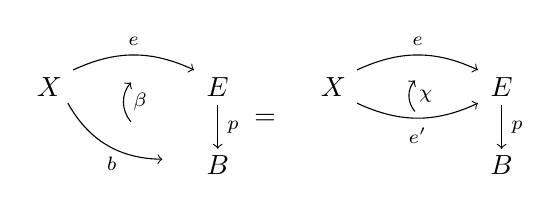
\begin{tikzpicture}[x=1.9em,y=1.5em]
  \node (X) at (0,0)     {$X$};
  \node (E) at (3.2,0)   {$E$};
  \node (B) at (3.2,-1.9){$B$};
  \draw[->] (0.45,0.4) to[bend left=25] node[above,pos=0.5]{$\scriptstyle e$} (2.75,0.4);
  \draw[->] (0.35,-0.4) to[bend right=30] node[below,pos=0.55]{$\scriptstyle b$} (2.15,-1.75);
  \draw[->] (3.2,-0.45) -- node[right]{$\scriptstyle p$} (3.2,-1.5);
  \draw[->] (1.55,-0.85) to[bend left=40] node[right]{$\scriptstyle\beta$} (1.55,0.1);
  \node at (4.1,-0.8) {$=$};
  \begin{scope}[shift={(5.4,0)}]
    \node (X2) at (0,0)     {$X$};
    \node (E2) at (3.2,0)   {$E$};
    \node (B2) at (3.2,-1.9){$B$};
    \draw[->] (0.45,0.4) to[bend left=25] node[above,pos=0.5]{$\scriptstyle e$} (2.75,0.4);
    \draw[->] (0.45,-0.4) to[bend right=25] node[below,pos=0.5]{$\scriptstyle e'$} (2.75,-0.4);
    \draw[->] (3.2,-0.45) -- node[right]{$\scriptstyle p$} (3.2,-1.5);
    \draw[->] (1.55,-0.6) to[bend left=40] node[right]{$\scriptstyle\chi$} (1.55,0.15);
  \end{scope}
\end{tikzpicture}
\end{center}
并带有如下性质：
\begin{itemize}
\item \textbf{归纳}：给定任何\trFunctor{} $f\colon Y\to X$ 与自然变换
\scalebox{0.85}{\cellpair{Y}{E}{e''}{ef}{\tau}} 和 \scalebox{0.85}{\cellpair{Y}{B}{pe''}{pe'f}{\gamma}}，满足
$p\tau=p\chi f\cdot\gamma$，则存在 $\gamma$ 的一个提升
\scalebox{0.85}{\cellpair{Y}{E}{e''}{e'f}{\bar\gamma}}，使得 $\tau=\chi f\cdot\bar\gamma$。
\item \textbf{保守性}：$\chi$ 之任何限制的纤维化自同态皆可逆：若
\cellpair{Y}{E}{e'f}{e'f}{\zeta} 是任一自然变换，满足 $\chi f\cdot\zeta=\chi f$
且 $p\zeta=\mathrm{id}_{pe'f}$，则 $\zeta$ 可逆。
\end{itemize}
\item 如下左图所示的每个自然变换 $\beta\colon b\Rightarrow pe$ 都容有一个如下
右图所示的提升 $\chi\colon e'\Rightarrow e$：
\begin{center}
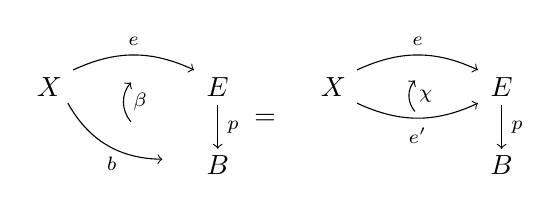
\begin{tikzpicture}[x=1.9em,y=1.5em]
  \node (X) at (0,0)     {$X$};
  \node (E) at (3.2,0)   {$E$};
  \node (B) at (3.2,-1.9){$B$};
  \draw[->] (0.45,0.4) to[bend left=25] node[above,pos=0.5]{$\scriptstyle e$} (2.75,0.4);
  \draw[->] (0.35,-0.4) to[bend right=30] node[below,pos=0.55]{$\scriptstyle b$} (2.15,-1.75);
  \draw[->] (3.2,-0.45) -- node[right]{$\scriptstyle p$} (3.2,-1.5);
  \draw[->] (1.55,-0.85) to[bend left=40] node[right]{$\scriptstyle\beta$} (1.55,0.1);
  \node at (4.1,-0.8) {$=$};
  \begin{scope}[shift={(5.4,0)}]
    \node (X2) at (0,0)     {$X$};
    \node (E2) at (3.2,0)   {$E$};
    \node (B2) at (3.2,-1.9){$B$};
    \draw[->] (0.45,0.4) to[bend left=25] node[above,pos=0.5]{$\scriptstyle e$} (2.75,0.4);
    \draw[->] (0.45,-0.4) to[bend right=25] node[below,pos=0.5]{$\scriptstyle e'$} (2.75,-0.4);
    \draw[->] (3.2,-0.45) -- node[right]{$\scriptstyle p$} (3.2,-1.5);
    \draw[->] (1.55,-0.6) to[bend left=40] node[right]{$\scriptstyle\chi$} (1.55,0.15);
  \end{scope}
\end{tikzpicture}
\end{center}
并带有如下性质：诱导映射是一条\trTrivialFibration{}
\[
E_{/\chi}\twoheadrightarrow B_{/\beta}\mathbin{\underset{B_{/pe}}{\times}}E_{/e}\text{。}
\]
\item 函子 $\Delta_{p}\colon E\to\mathrm{Hom}_{B}(B,p)$ 容有一个 $B$ 上的%
\trRightAdjoint。
\item 函子 $i_{1}\hat{p}\colon E^{2}\twoheadrightarrow\mathrm{Hom}_{B}(B,p)$
容有一个\trRightAdjoint\trRightInverse。
\item $B$ 中任何 1-\trSimplex{} $\beta\colon b\to pe$ 都容有 $E$ 中的一个提升
$\chi\colon e'\to e$，使得任何 $n\ge 1$ 的\trLifting{}问题
\begin{center}
\begin{tikzpicture}[x=1.9em,y=1.4em]
  \node (d1)  at (0,1.3)    {$\Delta[1]$};
  \node (pd)  at (3.9,1.3)  {$\partial\Delta[n]\times\Delta[1]$};
  \node (d11) at (8.1,1.3)  {$\Delta[n]\times\{1\}$};
  \node (E)   at (10.9,1.3) {$E$};
  \node (dn)  at (5.0,-1.4) {$\Delta[n]\times\Delta[1]$};
  \node (B)   at (10.9,-1.4){$B$};
  \draw[->] (0.9,1.3) -- node[below]{$\scriptstyle\{n\}\times\mathrm{id}$} (2.3,1.3);
  \draw[->] (6.1,1.3) -- (6.9,1.3);
  \draw[->] (9.4,1.3) -- (10.2,1.3);
  \node at (6.0,1.8) {$\scriptstyle\sqcup$};
  \node at (6.0,0.7) {$\scriptstyle\partial\Delta[n]\times\{1\}$};
  \draw[->] (1.0,1.9) to[bend left=18] node[above,pos=0.45]{$\scriptstyle\chi$} (10.3,1.9);
  \draw[right hook->] (5.0,0.95) -- (5.0,-0.9);
  \draw[->,dashed] (5.5,-1.2) -- (10.4,1.0);
  \draw[->] (10.9,0.95) -- node[right]{$\scriptstyle p$} (10.9,-0.9);
  \draw[->] (6.8,-1.4) -- (9.9,-1.4);
\end{tikzpicture}
\end{center}
都有解。
\item $B$ 中任何 1-\trSimplex{} $\beta\colon b\to pe$ 都容有 $E$ 中的一个提升
$\chi\colon e'\to e$，使得任何 $n\ge 2$ 的\trLifting{}问题
\begin{center}
\begin{tikzpicture}[x=1.9em,y=1.4em]
  \node (d1) at (0,1.3)    {$\Delta[1]$};
  \node (ho) at (3.6,1.3)  {$\Lambda^{n}[n]$};
  \node (E)  at (7.4,1.3)  {$E$};
  \node (dn) at (3.6,-1.4) {$\Delta[n]$};
  \node (B)  at (7.4,-1.4) {$B$};
  \draw[->] (1.0,1.3) -- node[below]{$\scriptstyle\{n-1,n\}$} (2.6,1.3);
  \draw[->] (4.6,1.3) -- (6.4,1.3);
  \draw[->] (0.6,1.8) to[bend left=20] node[above,pos=0.5]{$\scriptstyle\chi$} (6.8,1.8);
  \draw[right hook->] (3.6,0.95) -- (3.6,-0.9);
  \draw[->,dashed] (4.0,-1.2) -- (6.9,1.0);
  \draw[->] (7.4,0.95) -- node[right]{$\scriptstyle p$} (7.4,-0.9);
  \draw[->] (4.6,-1.4) -- (6.4,-1.4);
\end{tikzpicture}
\end{center}
都有解。
\end{enumerate}
\end{proposition}

条件 (vi) 看似比 \cite[2.4.2.1]{bib78} 略强——后者只要求 $p$ 是一个带有
(F.4.2) 之\trLifting{}性质的\trInnerFibration（inner fibration）——但不难推知：任何
这样的 $p$ 必是一条\trIsofibration（见\cref{ex:inner-fibration-isofibration}）。

\begin{proof}
(i) 与 (iii) 的等价性证明于\cref{prop:external-characterization}，其中用到
\cref{prop:cartesian-arrow-analytic}中 (i) 等价于 (iv) 的事实来鉴别刻画
$p$-\trCartesianArrow{}的那个等价；而 (ii)、(iii) 与 (iv) 的等价性则证明于
\cref{thm:internal-characterization}。

剩下要验证的，是这些综合条件与相应解析条件之间的等价性。我们将证明
(iv)$\Longleftrightarrow$(v) 与 (v)$\Longleftrightarrow$(vi)。

由\cref{lem:rajri-lifting}，\trIsofibration{} $i_{1}\hat{p}$ 容有一个%
\trRightAdjoint\trRightInverse，当且仅当 $B$ 中任何 1-\trSimplex{}
$\beta\colon b\to pe$ 都容有 $E$ 中的一个提升 $\chi\colon e'\to e$，使得任何
$n\ge 1$ 的如下\trLifting{}问题
\begin{center}
\begin{tikzpicture}[x=1.9em,y=1.4em]
  \node (o)  at (0,1.3)    {$1$};
  \node (pd) at (3.4,1.3)  {$\partial\Delta[n]$};
  \node (E2) at (7.0,1.3)  {$E^{2}$};
  \node (dn) at (3.4,-1.4) {$\Delta[n]$};
  \node (H)  at (7.0,-1.4) {$\mathrm{Hom}_{B}(B,p)$};
  \draw[->] (0.4,1.3) -- node[below]{$\scriptstyle\{n\}$} (2.5,1.3);
  \draw[->] (4.3,1.3) -- (6.1,1.3);
  \draw[->] (0.5,1.8) to[bend left=20] node[above,pos=0.5]{$\scriptstyle\chi$} (6.4,1.8);
  \draw[right hook->] (3.4,0.95) -- (3.4,-0.9);
  \draw[->,dashed] (3.8,-1.2) -- (6.4,1.0);
  \draw[->] (7.0,0.95) -- node[right]{$\scriptstyle i_{1}\hat{p}$} (7.0,-0.9);
  \draw[->] (4.3,-1.4) -- (5.7,-1.4);
\end{tikzpicture}
\end{center}
都有解。这一\trLifting{}性质等价于经转置的\trLifting{}性质
\begin{center}
\begin{tikzpicture}[x=1.9em,y=1.4em]
  \node (d1)  at (0,1.3)    {$\Delta[1]$};
  \node (pd)  at (3.9,1.3)  {$\partial\Delta[n]\times\Delta[1]$};
  \node (d11) at (8.1,1.3)  {$\Delta[n]\times\{1\}$};
  \node (E)   at (10.9,1.3) {$E$};
  \node (dn)  at (5.0,-1.4) {$\Delta[n]\times\Delta[1]$};
  \node (B)   at (10.9,-1.4){$B$};
  \draw[->] (0.9,1.3) -- node[below]{$\scriptstyle\{n\}\times\mathrm{id}$} (2.3,1.3);
  \draw[->] (6.1,1.3) -- (6.9,1.3);
  \draw[->] (9.4,1.3) -- (10.2,1.3);
  \node at (6.0,1.8) {$\scriptstyle\sqcup$};
  \node at (6.0,0.7) {$\scriptstyle\partial\Delta[n]\times\{1\}$};
  \draw[->] (1.0,1.9) to[bend left=18] node[above,pos=0.45]{$\scriptstyle\chi$} (10.3,1.9);
  \draw[right hook->] (5.0,0.95) -- (5.0,-0.9);
  \draw[->,dashed] (5.5,-1.2) -- (10.4,1.0);
  \draw[->] (10.9,0.95) -- node[right]{$\scriptstyle p$} (10.9,-0.9);
  \draw[->] (6.8,-1.4) -- (9.9,-1.4);
\end{tikzpicture}
\end{center}
仍是对 $n\ge 1$ 而言，这就证明了 (iv) 与 (v) 之间的等价性。最后，
\cref{prop:cartesian-arrow-analytic}(v)$\Longleftrightarrow$(vi) 证明了 (vi) 与 (v) 之间的
等价性。
\end{proof}

现在我们把\trCartesianArrow{}的概念加以扩充，定义一个「笛卡尔柱面」（cartesian
cylinder）概念，用以描述\cref{prop:cartesian-arrow-analytic}中出现的诸%
\trLifting{}性质的一个变体。

\begin{definition}[笛卡尔柱面]\label{def:cartesian-cylinders}
设 $p\colon E\twoheadrightarrow B$ 是拟范畴之间的一条\trCartesianFibration，
并设 $X$ 是任意\trSimplicialSet。我们称一个柱面 $e\colon X\times\Delta[1]\to E$
是\textbf{逐点 $p$-\trCartesian}（pointwise $p$-cartesian），当且仅当对每个
0-\trSimplex{} $x\in X$，$e$ 把 1-\trSimplex{}
$(x\sigma^{0},\mathrm{id}_{[1]})\colon(x,0)\to(x,1)$ 送到 $E$ 中的一支
$p$-\trCartesianArrow。
\end{definition}

\begin{lemma}\label{lem:pointwise-pcartesian-cylinder}
设 $p\colon E\twoheadrightarrow B$ 是拟范畴之间的一条\trCartesianFibration。
柱面 $e\colon X\times\Delta[1]\to E$ 是逐点 $p$-\trCartesian{}，当且仅当
$e\colon\Delta[1]\to E^{X}$ 为笛卡尔纤维化
$p^{X}\colon E^{X}\twoheadrightarrow B^{X}$ 定义了一支 $p^{X}$-\trCartesianArrow。
\end{lemma}

\begin{proof}
首先注意，\cref{cor:cosmological-functors-preserve-cartesian}蕴含
$p^{X}\colon E^{X}\twoheadrightarrow B^{X}$ 是一条\trCartesianFibration，而
\cref{prop:cartesian-representable}则证明：沿任何 $f\colon Y\to X$ 的限制定义
出诸\trCartesianFibration{}之间的一个笛卡尔函子
\begin{center}
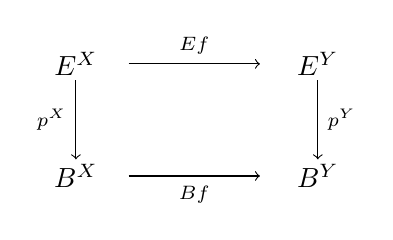
\begin{tikzpicture}[x=1.9em,y=1.5em]
  \node (EX) at (0,1.3)  {$E^{X}$};
  \node (EY) at (4.6,1.3){$E^{Y}$};
  \node (BX) at (0,-1.4) {$B^{X}$};
  \node (BY) at (4.6,-1.4){$B^{Y}$};
  \draw[->] (1.0,1.3) -- node[above]{$\scriptstyle Ef$} (3.5,1.3);
  \draw[->] (0,0.9) -- node[left]{$\scriptstyle p^{X}$} (0,-1.0);
  \draw[->] (4.6,0.9) -- node[right]{$\scriptstyle p^{Y}$} (4.6,-1.0);
  \draw[->] (1.0,-1.4) -- node[below]{$\scriptstyle Bf$} (3.5,-1.4);
\end{tikzpicture}
\end{center}
特别地，$p^{X}$-\trCartesianArrow{}都是逐点 $p$-笛卡尔的。反之，任何逐点 $p$-笛卡尔
柱面都经由一个逐点同构穿过一支 $p^{X}$-\trCartesianArrow{}而分解。由
\cref{cor:exponential-ideal}，逐点同构实际上就是同构，故由 $p^{X}$-\trCartesianArrow{}%
的同构稳定性，任何逐点 $p$-笛卡尔柱面都是一支 $p^{X}$-\trCartesianArrow。
\end{proof}

下述\trLifting{}性质将用于证明\cref{prop:cocartesian-rari-terminal-elements}。

\begin{lemma}\label{lem:cylinder-lifting-property}
设 $X\hookrightarrow Y$ 是单纯集 $Y$ 的一个单纯子集。
\begin{enumerate}[label=(\roman*)]
\item 任何 $n\ge 0$ 的\trLifting{}问题
\begin{center}
\begin{tikzpicture}[x=1.9em,y=1.4em]
  \node (u) at (0,1.3)    {$X\times\Delta[1]\cup Y\times\{1\}$};
  \node (E) at (7.0,1.3)  {$E$};
  \node (l) at (0,-1.4)   {$Y\times\Delta[1]$};
  \node (B) at (7.0,-1.4) {$B$};
  \draw[->] (3.6,1.3) -- node[above]{$\scriptstyle e$} (6.2,1.3);
  \draw[right hook->] (0,0.9) -- (0,-1.0);
  \draw[->,dashed] (0.8,-1.2) -- (6.2,1.05);
  \node at (3.4,-0.4) {$\scriptstyle\bar{e}$};
  \draw[->] (7.0,0.95) -- node[right]{$\scriptstyle p$} (7.0,-1.0);
  \draw[->] (2.6,-1.4) -- node[below]{$\scriptstyle b$} (5.6,-1.4);
\end{tikzpicture}
\end{center}
其中柱面
$X\times\Delta[1]\subseteq X\times\Delta[1]\cup Y\times\{1\}\xrightarrow{\ e\ }E$
是逐点 $p$-笛卡尔的，都容有一个解 $\bar{e}$，且该解同样是逐点 $p$-笛卡尔的。
\item 任何 $n\ge 1$ 的\trLifting{}问题
\begin{center}
\begin{tikzpicture}[x=1.9em,y=1.4em]
  \node (u) at (0,1.3)    {$X\times\Delta[n]\cup Y\times\Lambda^{n}[n]$};
  \node (E) at (7.0,1.3)  {$E$};
  \node (l) at (0,-1.4)   {$Y\times\Delta[n]$};
  \node (B) at (7.0,-1.4) {$B$};
  \draw[->] (4.3,1.3) -- node[above]{$\scriptstyle e$} (6.2,1.3);
  \draw[right hook->] (0,0.9) -- (0,-1.0);
  \draw[->,dashed] (0.8,-1.2) -- (6.2,1.05);
  \node at (3.4,-0.4) {$\scriptstyle\bar{e}$};
  \draw[->] (7.0,0.95) -- node[right]{$\scriptstyle p$} (7.0,-1.0);
  \draw[->] (2.4,-1.4) -- node[below]{$\scriptstyle b$} (5.6,-1.4);
\end{tikzpicture}
\end{center}
其中柱面
$Y\times\Delta^{\{n-1,n\}}\subseteq X\times\Delta[n]\cup Y\times\Lambda^{n}[n]\xrightarrow{\ e\ }E$
是逐点 $p$-笛卡尔的，都容有一个解 $\bar{e}$。
\end{enumerate}
\end{lemma}

\begin{proof}
带 $X\hookrightarrow Y$ 的\trLeibnizTensor{}定义了一个函子
$\sSet^{2}\to\sSet^{2}$，它保持收缩图 \eqref{eq:horn-inclusion-retract}，故
(ii) 的\trLifting{}性质由 (i) 得出。而 (i) 的\trLifting{}性质则归纳地由
\cref{prop:cartesian-arrow-analytic}(vi) 结合「任何单态射 $X\hookrightarrow Y$
都可以分解为诸包含 $i_{n}\colon\partial\Delta[n]\hookrightarrow\Delta[n]$ 之
余积的推出的一个序列复合」这一事实得出；并且由
\cref{prop:leibniz-construction-preserves}(vii)，再与
$\{1\}\hookrightarrow\Delta[1]$ 作推出积，便同样给出诸推出积
$\partial\Delta[n]\times\Delta[1]\cup\Delta[n]\times\{1\}\hookrightarrow\Delta[n]\times\Delta[1]$
之余积的推出的一个序列复合。
\end{proof}

最后一个结果表明，拟范畴之间的\trDiscreteCocartesianFibration{}与\trDiscreteCartesianFibration，分别与
Joyal \cite{bib61} 所引入的\trLeftFibration{}类与\trRightFibration{}类相重合。

\begin{proposition}\label{prop:discrete-cartesian-analytic}
对拟范畴之间的一条\trIsofibration{} $p\colon E\twoheadrightarrow B$，以下诸
条件等价，并且定义了 $p$ 成为一条\textbf{\trDiscreteCartesianFibration}的含义：
\begin{enumerate}[label=(\roman*)]
\item 映射 $p\colon E\twoheadrightarrow B$ 是一条\trCartesianFibration，其诸%
\trFiber{}皆为\trKanComplex。
\item \trQuasiCategory{}的\trHomotopyTwoCategory{}中的每个 2-\trCell{}
$\beta\colon b\Rightarrow pe$ 都容有一个本质唯一的提升：给定
$\chi\colon e'\Rightarrow e$ 与 $\psi\colon e''\Rightarrow e$ 使得
$p\chi=p\psi=\beta$，则存在一个\trIsomorphism{} $\gamma\colon e''\Rightarrow e'$，
使得 $\chi\cdot\gamma=\psi$ 且 $p\gamma=\mathrm{id}$。
\item 诱导函子 $i_{1}\hat{p}\colon E^{2}\twoheadrightarrow\mathrm{Hom}_{B}(B,p)$
是一条\trTrivialFibration。
\item 函子 $p\colon E\to B$ 是一个\trRightFibration，即带有如下\trLifting{}性质：
\begin{center}
\begin{tikzpicture}[x=1.9em,y=1.4em]
  \node (ho) at (0,1.3)   {$\Lambda^{k}[n]$};
  \node (E)  at (3.6,1.3) {$E$};
  \node (dn) at (0,-1.4)  {$\Delta[n]$};
  \node (B)  at (3.6,-1.4){$B$};
  \draw[->] (1.0,1.3) -- (2.8,1.3);
  \draw[right hook->] (0,0.95) -- (0,-0.9);
  \draw[->,dashed] (0.45,-1.2) -- (3.1,1.05);
  \draw[->] (3.6,0.95) -- node[right]{$\scriptstyle p$} (3.6,-1.0);
  \draw[->] (1.0,-1.4) -- (2.8,-1.4);
  \node at (6.1,0) {对 $n\ge 0$ 与 $0<k\le n$。};
\end{tikzpicture}
\end{center}
\end{enumerate}
\end{proposition}

\begin{proof}
第一个刻画 (i) 是把原来的\cref{def:discrete-co-cartesian-fibration}借
\cref{prop:discrete-fibers-isofibration}重新解读——后者说：一条\trIsofibration{}
$p\colon E\twoheadrightarrow B$ 在 $\QCat_{/B}$ 中定义一个\trDiscrete{}对象，
当且仅当其诸\trFiber{}是\trKanComplex。(i) 与 (ii) 的等价性证明于
\cref{prop:discrete-cartesian-characterization}，而 (i) 与 (iii) 的等价性则
证明于\cref{prop:internal-characterization-discrete}。

我们最后证明 (iii) 与 (iv) 的等价性。经伴随，$i_{1}\hat{p}$ 是一条%
\trTrivialFibration，当且仅当如下右方的\trLifting{}问题有解
\begin{center}
\begin{tikzpicture}[x=1.9em,y=1.4em]
  \node (pd) at (0,1.3)    {$\partial\Delta[n]$};
  \node (E2) at (3.4,1.3)  {$E^{2}$};
  \node (dn) at (0,-1.4)   {$\Delta[n]$};
  \node (H)  at (3.4,-1.4) {$\mathrm{Hom}_{B}(B,p)$};
  \draw[->] (1.0,1.3) -- (2.3,1.3);
  \draw[right hook->] (0,0.95) -- (0,-0.9);
  \draw[->,dashed] (0.5,-1.2) -- (2.9,1.05);
  \draw[->] (3.4,0.95) -- node[right]{$\scriptstyle i_{1}\hat{p}$} (3.4,-1.0);
  \draw[->] (1.0,-1.4) -- (2.1,-1.4);
  \node at (5.2,0) {$\;\leftrightsquigarrow\;$};
  \begin{scope}[shift={(7.8,0)}]
    \node (u) at (0,1.3)    {$\partial\Delta[n]\times\Delta[1]\cup\Delta[n]\times\{1\}$};
    \node (E) at (6.6,1.3)  {$E$};
    \node (l) at (0,-1.4)   {$\Delta[n]\times\Delta[1]$};
    \node (B) at (6.6,-1.4) {$B$};
    \draw[->] (4.6,1.3) -- (5.8,1.3);
    \draw[right hook->] (0,0.9) -- (0,-1.0);
    \draw[->,dashed] (0.8,-1.2) -- (5.9,1.05);
    \draw[->] (6.6,0.95) -- node[right]{$\scriptstyle p$} (6.6,-1.0);
    \draw[->] (3.0,-1.4) -- (5.4,-1.4);
  \end{scope}
\end{tikzpicture}
\end{center}
由\cref{prop:leibniz-marked-anodyne}，若 $p\colon E\to B$ 是一个满足条件 (iv)
的\trRightFibration，则如上右方的\trLifting{}问题容有一个解，从而
$i_{1}\hat{p}\colon E^{2}\twoheadrightarrow\mathrm{Hom}_{B}(B,p)$ 是一条%
\trTrivialFibration，即证得 (iii)。反之，对 $0<k\le n$，号角包含
$\Lambda^{k}[n]\hookrightarrow\Delta[n]$ 是一个收缩
\begin{center}
\begin{tikzpicture}[x=1.9em,y=1.5em]
  \node (a) at (0,1.3)    {$\Lambda^{k}[n]$};
  \node (b) at (5.0,1.3)  {$\Lambda^{k}[n]\times\Delta[1]\cup\Delta[n]\times\{1\}$};
  \node (c) at (11.4,1.3) {$\Lambda^{k}[n]$};
  \node (d) at (0,-1.6)   {$\Delta[n]$};
  \node (e) at (5.0,-1.6) {$\Delta[n]\times\Delta[1]$};
  \node (f) at (11.4,-1.6){$\Delta[n]$};
  \draw[right hook->] (1.0,1.3) -- node[above]{$\scriptstyle\Lambda^{k}[n]\times\{0\}$} (2.4,1.3);
  \draw[->] (8.4,1.3) -- node[above]{$\scriptstyle r$} (10.3,1.3);
  \draw[right hook->] (1.0,-1.6) -- node[above]{$\scriptstyle\Delta[n]\times\{0\}$} (2.9,-1.6);
  \draw[->] (7.6,-1.6) -- node[above]{$\scriptstyle r$} (10.3,-1.6);
  \draw[right hook->] (0,0.9) -- (0,-1.1);
  \draw[right hook->] (5.0,0.8) -- (5.0,-1.1);
  \draw[right hook->] (11.4,0.9) -- (11.4,-1.1);
\end{tikzpicture}
\end{center}
其中 $r(i,0)=i$，而
$r(i,1)=\begin{cases}i & i\ne k-1\\ k & i=k-1\end{cases}$。于是，要求解 (iv)
所假定的那一\trLifting{}问题，只需证明 $p$ 对推出积
$(\Lambda^{k}[n]\hookrightarrow\Delta[n])\mathbin{\widehat{\times}}(\{1\}\hookrightarrow\Delta[1])$
容有提升；而后者经转置便成为单态射
$\Lambda^{k}[n]\hookrightarrow\Delta[n]$ 与
$i_{1}\hat{p}\colon E^{2}\twoheadrightarrow\mathrm{Hom}_{B}(B,p)$ 之间的一个%
\trLifting{}问题。若 (iii) 成立且 $i_{1}\hat{p}$ 是一条\trTrivialFibration，
那么这就构造出所求的提升。
\end{proof}

\subsection*{练习}

\begin{exercise}\label{ex:inner-fibration-isofibration}
设 $p\colon E\to B$ 是拟范畴之间的一个\trInnerFibration，使得 $B$ 中任何 1-\trSimplex{}
$\beta\colon b\to pe$ 都容有 $E$ 中的一个提升 $\chi\colon e'\to e$，使得任何
$n\ge 2$ 的\trLifting{}问题
\begin{center}
\begin{tikzpicture}[x=1.9em,y=1.4em]
  \node (d1) at (0,1.3)    {$\Delta[1]$};
  \node (ho) at (3.6,1.3)  {$\Lambda^{n}[n]$};
  \node (E)  at (7.4,1.3)  {$E$};
  \node (dn) at (3.6,-1.4) {$\Delta[n]$};
  \node (B)  at (7.4,-1.4) {$B$};
  \draw[->] (1.0,1.3) -- node[below]{$\scriptstyle\{n-1,n\}$} (2.6,1.3);
  \draw[->] (4.6,1.3) -- (6.4,1.3);
  \draw[->] (0.6,1.8) to[bend left=20] node[above,pos=0.5]{$\scriptstyle\chi$} (6.8,1.8);
  \draw[right hook->] (3.6,0.95) -- (3.6,-0.9);
  \draw[->,dashed] (4.0,-1.2) -- (6.9,1.0);
  \draw[->] (7.4,0.95) -- node[right]{$\scriptstyle p$} (7.4,-0.9);
  \draw[->] (4.6,-1.4) -- (6.4,-1.4);
\end{tikzpicture}
\end{center}
都有解。证明 $p$ 是一个\trIsofibration。
\end{exercise}

\begin{exercise}\label{ex:cocartesian-equivalences}
陈述并证明下述诸对象的多种综合定义与解析定义之间的等价：
\begin{enumerate}[label=(\roman*)]
\item 拟范畴之间的一条余笛卡尔纤维化；
\item 拟范畴中的一支\trCocartesianArrow（cocartesian arrow）；
\item 拟范畴之间的一条\trDiscreteCocartesianFibration。
\end{enumerate}
\end{exercise}

